%% bare_conf.tex
%% V1.4b
%% 2015/08/26
%% by Michael Shell
%% See:
%% http://www.michaelshell.org/
%% for current contact information.
%%
%% This is a skeleton file demonstrating the use of IEEEtran.cls
%% (requires IEEEtran.cls version 1.8b or later) with an IEEE
%% conference paper.
%%
%% Support sites:
%% http://www.michaelshell.org/tex/ieeetran/
%% http://www.ctan.org/pkg/ieeetran
%% and
%% http://www.ieee.org/

\documentclass[10pt, conference, letterpaper]{IEEEtran}

% Imported pakcages

\usepackage{url}
\usepackage{listings}
\usepackage{booktabs}
%\usepackage{subfigure}
\usepackage{threeparttable}
\usepackage{todonotes}
\usepackage{cite}
\usepackage{graphicx}
\usepackage{algpseudocode}
\usepackage{color,colortbl}
\usepackage{soul}
\usepackage{stfloats}
%\usepackage{subfig}
\usepackage{xspace}
\usepackage{multirow}
\usepackage{subcaption}
\usepackage{flushend}

%\usepackage[margin=5pt]{caption}
\usepackage{lstlangarm}
\newcolumntype{L}[1]{>{\raggedright\let\newline\\\arraybackslash}m{#1}}
\newcolumntype{C}[1]{>{\centering\let\newline\\\arraybackslash}m{#1}}
\newcolumntype{R}[1]{>{\raggedleft\let\newline\\\arraybackslash}m{#1}}

\graphicspath{ {./figs/}}

\lstset{breaklines}
\hyphenation{op-tical net-works semi-conduc-tor}
\lstset{
keywordstyle=\bfseries\color{blue},
stringstyle=\color{olive},
basicstyle=\footnotesize\ttfamily,
rulecolor=\color{black},
numbers=left,
extendedchars=false
numberstyle=\tiny,
commentstyle=\itshape\color{black},
showstringspaces=false,
frame=single,
xleftmargin=1.5em,
xrightmargin=1.5em,
captionpos=b
}

\graphicspath{ {./figs/}}

% Commands
\newcommand{\tabincell}[2]{\begin{tabular}{@{}#1@{}}#2\end{tabular}}
\newcommand{\sysname}{AFL-IoT\xspace}

\begin{document}

%don't want date printed
\date{}

%make title bold and 14 pt font (Latex default is non-bold, 16 pt)
\title{\Large \bf  \sysname : Fuzzing on Linux-based IoT Device with Binary Level Instrumentation}

\author{Anonymous Submission}



%%for single author (just remove % characters)
%\author{
%{\rm Your N.\ Here}\\
%Your Institution
%\and
%{\rm Second Name}\\
%Second Institution
%% copy the following lines to add more authors
%% \and
%% {\rm Name}\\
%%Name Institution
%} % end author

\maketitle

% Use the following at camera-ready time to suppress page numbers.
% Comment it out when you first submit the paper for review.
\thispagestyle{empty}
\pagestyle{plain}

\begin{abstract}
With the growing prevalence of Internet of Things~(IoT), security and privacy issues on IoT devices have considerably increased. Due to limited resources, security analysis on IoT devices faces great challenges. On one hand, even though there are several existing works that provide automated solutions to identifying vulnerabilities on IoT devices, they are either inaccurate or not scalable. On the other hand, although sophisticated fuzzing technique has been studied for decades and has proved itself to be very effective in solving the aforementioned problems to find software bugs, none of existing fuzzing approaches could work on IoT devices. 

In this paper, we present \sysname, the first lightweight and deployable fuzzing framework for Linux-based IoT devices. Using binary level instrumentation, \sysname executes the instrumented binary program directly on IoT devices during the fuzzing process. We evaluated \sysname on both benchmarks and real world IoT devices. In total, \sysname identified 157 unique crashes in 10 binary programs with only 10\% performance overhead on average, showing that it is both efficient and effective to find software bugs in binary programs on Linux-based IoT devices.

\end{abstract}
\section{Introduction}\label{sec:intro}

Although it has been decades since the concept of Internet of Things~(IoT) was first presented~\cite{wikiiot}, only in recent years have we witnessed an outbreak of its application in our daily life. Various types of Commercial-Off-The-Shelf~(COTS) IoT devices emerged rapidly, such as IP cameras, home routers, printers, smart TVs, lamps, fridges and air-conditioners. These devices extend the Internet connectivity beyond traditional devices~(e.g. computers and smartphones) to any object we may use. Thus, it greatly expands the capability of the Internet and provides convenience for everyone.

However, the widespread application of IoT devices also brings new challenges for security and privacy. Interconnection of these devices that were originally isolated from each other significantly expands the attacking surface and thus makes IoT devices more vulnerable to cyber-attacks. For example, privilege escalation vulnerabilities have been found in smart lock and can be used by attackers to break the authentication~\cite{lock}. Even worse, security researchers~\cite{nie2017free} have demonstrated that it is possible to penetrate into a car and gain remote control of Engine Control Units~(ECU) simply with the help a phishing WiFi hotspot. Without physical access, both attacks were considered impossible in the past. Moreover, compared with traditional devices like smartphone, IoT devices often have relatively limited hardware resources and thus usually lack security mechanisms to prevent various attacks due to performance concern. That makes IoT devices even more exploitable.

To mitigate aforementioned security issues, many existing works attempted to find software vulnerabilities and flaws in IoT devices. Costin et al.~\cite{costin2014large} leveraged static analysis techniques to automatically acquire and analyze a large number of firmwares. They used specific patterns to search for existing security flaws in these firmwares. Although this approach is lightweight and scalable, it suffers from the inherited limitation of static analysis: accuracy.

Zaddach et al.~\cite{zaddach2014avatar} however took a dynamic approach to conduct security analysis on IoT devices by monitoring the firmwares execution on a hybrid system combining both emulator and real IoT hardware. The hybrid system automatically forwards all I/O accesses from the emulator to the real device and therefore precisely emulates the execution of the firmware. While this approach may be accurate, it still suffers from efficiency and scalability issues. Chen et al.~\cite{chen2016towards} designed a dynamic analysis system for Linux-based IoT device's firmware. It takes an emulator-based approach to identify software vulnerabilities by performing large scale automated black-box testing with web exploits. Unfortunately, emulating various types of IoT devices is a non-trivial task. Their approach failed to resolve many dependencies such as a specific version of Linux kernel or certain kind of kernel modules before the OS can actually boot. Such failures may cause a large number of kernel panics during the emulation, which decreases the effectiveness of their approach. 

To overcome the limitations of existing work, we take a different approach by using fuzzing in the security analysis of Linux-based IoT devices. Fuzzing is an effective technique to find software bugs. For example, AFL~\cite{aflweb} is a well-known coverage-based gray-box fuzzer~(or fuzzer), which mutates the input to trigger bugs in the target program. AFL has identified a large number of security vulnerabilities in many popular open source projects. However, although fuzzing has been studied in the field of software security for years, even today we still rarely see its application in IoT devices. 


Compared with its application on x86 platforms, fuzzing on IoT devices poses the following major challenges: 

\begin{enumerate}
\item \textbf{No source code.} Commercial-off-the-shelf (COTS) IoT devices are usually installed with many proprietary software. Generally, source code and documentation of such software are unavailable. All existing solutions for binary program fuzzing require runtime emulation, which is non-trivial on IoT devices. %So it is difficult to apply coverage-based fuzzing techniques in these software. 

\item \textbf{Limited resources.} In comparison with x86 platform, IoT devices often have limited resource in terms of CPU, memory and storage. So lightweight analysis is required on IoT devices. Trade-off between accuracy and efficiency must be taken into consideration in system design and implementation.
\item \textbf{Network daemon programs.} Compared with most x86 platform devices, network daemon programs are more common on IoT devices, and sometimes even outnumber command line programs. These daemon programs take input from a network interface rather than a file or the standard input. Since traditional fuzzers can mutate only files or the standard input, we must design mechanisms to allow them to interact with daemon programs.  

%Besides, it requires additional migration and optimization work to integrate a fuzzer with the IoT device. 

%Consequently, there must be a trade-off between accuracy and efficiency when it comes to the system design, otherwise the fuzzing will be infeasible. 

%\item \textbf{No debug interface.} For security concerns, debug interface~(e.g. shell access) is usually disabled in most of COTS IoT devices, which makes it difficult to fuzzing on the target device.

%\item \textbf{\hl{Fuzzer integration.}} Unlike x86 platform, CPU architecture/instruction, operating system and tool-chain vary greatly in different IoT devices. Such differences bring significant challenges to fuzzer integration. 

\end{enumerate}

Despite of many existing works~\cite{rawat2017vuzzer, bohme2017coverage, cadar2008klee, stephens2016driller, godefroid2012sage, godefroid2005dart, sen2005cute, cha2015program, haller2013dowsing, ganesh2009taint, wang2010taintscope, bastani2017synthesizing, godefroid2017learn, wang2017skyfire} focusing on research of various fuzzing tools, all of them fail to address these challenges. Consequently, unlike all these works, our goal is to propose a novel approach to adapt existing fuzzer to work with binary programs on IoT devices for efficient and comprehensive security analysis. 


To this end, in this paper we design and implement \sysname, a lightweight and easy deployable coverage-based fuzzing framework for Linux-based IoT devices. \sysname extends AFL by implementing binary level instrumentation, so it can support native execution of the target binary program and therefore significantly reduces the performance overhead. In this way, \sysname makes it possible to directly fuzz binary program on IoT devices instead of expensive runtime emulation and therefore addresses the first challenge.

Considering the limited resources on IoT devices, our solution consists of two phases for each target binary program in fuzzing: 1) Instrumentation phase. 2) Fuzzing phase. As shown in Figure~\ref{figs:arch}, \sysname first completes the instrumentation phase on a powerful Linux server and then deploys the instrumented program with the fuzzer on the IoT device. Our two phase design significantly eases the burden of IoT devices and thus addresses the second challenge.   

%\sysname also provides capability of fuzzing on network daemon programs which usually makes up the majority of software on most Linux-based IoT devices. Unlike a command-line program, a network daemon program in general only take meaningful input from network interfaces.

Besides, our design also provides solutions to fuzzing on network daemon programs. Specifically, \sysname can forward all input from a fuzzer to a specific network interface which the target daemon program listens on. Such forwarding is achieved through a series of hook operations on Linux socket APIs. In this way, \sysname avoids expensive network operations and thus makes it more efficient for fuzzing on network daemon programs, which definitely addresses the third challenge.

To our best knowledge, we are the first to provide a practical fuzzing solution to binary programs on Linux-based IoT devices. We evaluate \sysname on both benchmarks and real-world devices. Results shows that \sysname achieves nearly the same performance on binary program in comparison with programs that AFL compiles from the source code and only has 10\% performance overhead on average~(See Section~\ref{sec:eval:performance}). In contrast, the performance overhead of the emulation-based approach that originally implemented in AFL ranges from 100\% to 400\%~\cite{aflreadme}, which is obviously too expensive for most IoT devices. 

Overall, \sysname successfully identify 157 unique crashes in 10 binary programs on real-world Linux-based IoT devices in our evaluation~(See Section~\ref{sec:eval:real}), showing that the approach that we apply in \sysname is both efficient and effective to find software bugs in binary programs on Linux-based IoT devices. 

%To summarize, our paper makes the following contributions: 

%\begin{itemize}
% \item We present \sysname, a lightweight and easy deployable coverage-based fuzzing framework that targets at binary programs on Linux-based IoT devices. 
% 
% 
% \item Our design and implementation of \sysname addresses several major challenges of fuzzing binary programs on IoT devices, such as fuzzer integration~(Section~ \ref{sec:impl:integ}), binary level instrumentation for executable programs and library programs~(Section~\ref{sec:design:inst}) and input forwarding for network daemon programs ~(Section~\ref{sec:design:daemons}).
% \item 
 
 %We evaluate \sysname on both benchmark and real-world IoT device, which proves its efficiency and effectiveness in finding software bugs in binary programs. In all, \sysname successfully identify \hl{157} unique crashes in \hl{10} binary program on real-world Linux-based IoT devices
%\end{itemize}

The rest of this paper is organized as follow. Section~\ref{sec:background} provides relevant background of AFL. Section~\ref{sec:design} and Section~\ref{sec:impl} depict the system design and implementation of \sysname, respectively. Section~\ref{sec:eval} evaluates \sysname on both benchmarks and real-world IoT devices. Section~\ref{sec:limit} discuss the limitation of our work. Section~\ref{sec:related} introduces related works and Section~\ref{sec:con} conclude the paper.


%Compared with AFL's emulation-based solution which often suffers a 100\% to 400\% performance overhead and thus is infeasible on most IoT devices, \sysname achieves nearly the same execution performance on binary program and only

%in comparison with programs that AFL compiles from the source code~\ref{}. 

%2 to 5 times performance overhead

%

%Mitigation: 

%Existing work: static: \cite{costin}: dynamic: \cite{Zaddach}, \cite{firmadyne} %have made their effort to mitigate security flaws: 
%explain their work:
%limitation: 
%Costin: validate security policies or properties 

%AVATAR: not efficient involving both hardware devices 

%FIRMADYNE: black-box emulator based approach, unable to resolve dependencies like kernel module, kernel version, focus on very limited existing exploits for penetration test, not accurate.


%Fuzzing 
%Main Challenges
%Our approach
%Our Contribution

% our contribution is on binary-level instrumentation, not fuzzer. Our approach can be applied to many existing fuzzing approach.

\section{Background}\label{sec:background}

\subsection{American Fuzzy Lop~(AFL)}
American Fuzzing Lop (AFL)~\cite{aflweb} is a famous coverage-based grey-box fuzzer which has been widely used to find software bugs in both academia and industry.  Although its approach seems to be ``naive'  which simply makes mutations based on the origin input (seed) and keeps track of the execution of target program by using lightweight instrumentation, it has been proved to be very efficient and effective. AFL has gain a good reputation by identifying a large number of unknown bugs~\cite{aflweb} in many popular opensource software projects. Next, we will go through some technique details to show basic ideas behind its design. 

\subsubsection{\bf{Branch Coverage}}

As a coverage-based gray-box fuzzer, AFL monitors the execution of the target program during the fuzzing process. Specifically, for each run of the target program, AFL maintains a 64KB map $shared\_mem[key]$ to keep track of the branch coverage information. It first generates a unique ID~($cur\_location$) for each basic block during the compilation and then instruments a small piece of code at each branch point to manipulate the map. If a certain basic block is hit during the execution, the instrumented code in this basic block increases the counter in \texttt{$shared\_mem[cur\_location \oplus prev\_location]$} by 1 where $prev\_location$ is the shifted ID of the basic block that hit before the branch point. To distinguish the execution order between two basic blocks, the instrumented code right shifts $cur\_location$ by 1 bit before assigns it to $pre\_location$~($pre\_location = cur\_location >> 1$). In this way, the entire execution path is recorded during each run of the target program and therefore AFL is capable of identifying new behaviors or internal states by comparing the executions paths that triggered by different inputs. All mutated inputs that can trigger new internal states within the target program are added to the input queue for further mutation in next runs, otherwise they are discarded. With the help of coverage-based guided fuzzing that described above, AFL is capable of exploring as many internal states of the target programs as possible, which significant increases the chance of finding bugs. 

\subsubsection{\bf{Target Instrumentation}}

The coverage measurement in AFL is implemented by instrumenting the target programs. Generally, such instrumentation is done during compilation and therefore requires source code of the target program. AFL provides two instrumentation approaches: assembly-level instrumentation and compiler-level instrumentation. The main difference is that the compiler-level instrumentation is performed on LLVM intermediate representation (IR) rather than manually instrumenting assembly code.  Such LLVM-based instrumentation has several advantages: 1.  It  benefits from many optimization features that provided by the compiler so it is more efficient; 2. It is CPU-independent so it can be applied to fuzz on non-x86 platforms. Specifically, AFL provides wrappers for different compilers which can be used to replace the original compiler in the building script of the target program, so the instrumentation is done during the building process. However, both instrumentation approaches leverage on compilers it is necessary for AFL to rebuild the target program from the source.  

In addition, AFL also has the capability to fuzz on binary program without source code.  This feature is very useful when fuzzing many proprietary software and is implemented by leveraging on QEMU~\cite{qemu}, an emulator that allows runtime instrumentation. While this emulator-based approach is feasible when fuzzing on binary programs, it still suffers from a major limitation. Emulator-based solutions are usually expensive because the emulator itself consumes large amount of resources. Besides, the emulator-based runtime instrumentation also has performance cost, which can significantly slow down the execution speed of the target program by two to five times~\cite{aflreadme}. Such performance overhead is probably unacceptable in some cases especially when fuzzing large binary programs.

%\subsubsection{``Fork-Server'' Optimization}

%\subsubsection{\hl{AFL Workflow}}




\section{Design}\label{sec:design}

In this section, we present our system design of \sysname and discuss technical details we apply in \sysname.

%\subsection{Motivation} 
%
%Fuzzing has been proved to be an effective technique to find software bugs. However, although this technique has been widely used in software security for years, even today we still rarely see its application in the field of IoT security. 
%
%%[Why Fuzzing]?
%Previous solutions for security analysis in IoT device can be categorized based on different analysis approaches they take. For example, Costin et al.~\cite{costin2014large} leverage on static analysis techniques to automatically unpack a large number of firmwares and then search for specific patterns to find existing security flaws in them. On the contrary, Chen et al.~\cite{chen2016towards} design a dynamic analysis system for Linux-based IoT device's firmware. It takes an emulator-based approach to identify software vulnerabilities by performing large scale automated black-box testing with various existing exploits. While these solutions are efficient and scalable, they either suffer from accuracy issues due to inherited limitations of static analysis or lack compatibility with various types of IoT devices. \hl{More importantly, all these previous research focus on identifying existing software security flaws.}
%
%Consequently, our goal is to provide efficient and comprehensive security analysis in Linux-based IoT devices and search for unknown security bugs by adopting fuzzing techniques in binary programs. 

%\subsection{Challenges}
%
%As mentioned earlier, fuzzing on IoT devices poses the following major challenges in comparison with fuzzing on x86 platforms.
%
%\begin{enumerate}
%\item \textbf{Limited Resources.} In comparison with x86 platform, IoT devices often have very limited resource in terms of CPU, memory and storage. Generally, it requires additional migration and optimization work to integrate a fuzzer with the origin operating system. Consequently, there must be a trade-off between accuracy and efficiency when it comes to the system design, otherwise the fuzzing will be infeasible. 
%
%\item \textbf{No source code available.} Commercial-off-the-shelf (COTS) IoT devices are usually installed with many proprietary software. Generally, source code and documentation of such software are not available, which makes it difficult to apply coverage-based grey-box~\cite{} fuzzing techniques in these software. 
%
%\item \textbf{No shell access.} For security concerns, shell access from network is strictly forbidden in most COTS IoT devices, which makes it difficult to deploy fuzzer in the target IoT devices.
%
%\item \textbf{Various CPU architecture, instructions and tool-chains.} Unlike x86 platform, various types of CPUs with different architectures and instructions are used in the domain of IoT devices. Such differences bring significant challenges to binary-level program analysis and instrumentation. Besides there is also a rich diversity of tool-chains that developed for different CPU architecture, which inevitably increases the difficulties of fuzzing on IoT devices. 
%\end{enumerate}


\subsection{Approach Overview}

We design and implement {\sysname}, a fast, lightweight and easy deployable coverage-based fuzzing framework for binary programs on Linux-based IoT device. The primary goal of {\sysname} is to provide practical solution for security researchers to automatically analyze software on IoT devices where source code is usually unavailable.

Generally, there are several different approaches to implement coverage-based fuzzing on binary programs. The first approach that comes mind is to use virtual machine emulation. As mentioned in Section~\ref{sec:background}, AFL leverages QEMU to hook instructions at each branch point in order to track execution of the target binary program. In this way, it achieves runtime instrumentation without modifying the target binary program. While this approach can provide the most accurate branch coverage information, it is too expensive to apply in IoT devices.

The next approach we can easily think of is assembly-level instrumentation which leverage on a disassembler as well as an assembler. Compared with the original binary program, assembly-level instrumentation only produces a small runtime overhead and all data references and function pointer access can be easily resolved by assembler after the instrumentation. However, this approach requires very high accuracy for both disassembler and assembler, which could be very challenging, especially for large complex binary programs.

%which pose 

%Unfortunately, in practice there is no tool available that meets such requirement, especially on large complex binary programs.

%However, in practice there is no disassembler available which can meet that precision requirement

%The advantages of this approach are that the instrumentation overhead is small in comparison with the original program and all data references and function pointer accesses can be easily resolved during the instrumentation. 

%However, such advantages only hold when the disassembler can precisely recognize all of the instructions and data within the original binary program.
%Unfortunately, in practice there is no disassembler available which can meet that precision requirement especially on large complex binary programs. As a result, disassemblers are usually used as auxiliary tools in reverse engineering tasks and therefore assembly-level instrumentation is also infeasible.

{\bf Our Approach: Binary-level instrumentation.}
Considering the infeasibility of the above two approaches, we choose binary-level instrumentation in our design. That means to statically instrument the target binary program with binary code that tracks coverage information during the fuzzing process. In our approach, instrumented code is injected at each branch point to track the execution of each basic block. So, we first identify all basic blocks in the binary program, then inject binary code at the beginning of each basic block. In this way, our approach maintains all the code and data structures in the original program and therefore avoid breaking its code logic.

%Although some existing tools (e.g. afl~\cite{aflwhitepaper}) have already provide capability to fuzz binary programs on x86 platform by adopting virtualization technology, there are still two major challenges to fuzz binary programs in IoT device's firmware in Virtual Machine: 


%\begin{enumerate}
	%\item Unlike many x86 platforms, most of IoT devices often have very limited resources, so VM-based solution is too expensive and in most cases is not even applicable on IoT devices.
	%\item Binary programs in IoT device's firmware often require specific runtime environment or even additional hardware support (e.g. NVRAM), which are extremely challenging to emulate in a VM.
%\end{enumerate}


%As a consequence, instead of running the target binary program inside a VM, we take a more efficient approach by adopting binary level instrumentation techniques in our system design. 

Generally, our approach has the following advantages: 1) It is lightweight and achieves almost the equivalent efficiency with source-code-level instrumentation~(See Section~\ref{sec:eval:performance}). 2) It is compatible with many IoT devices because it fuzzes the target program on the original device and therefore does not require migration work such as environment configuration and dependence installation. 3) The accuracy of instrumentation will not affect the correctness of the target program execution. It will only affect the coverage information that are collected during the execution of the target program.



\begin{figure*}[htbp]
\centering 
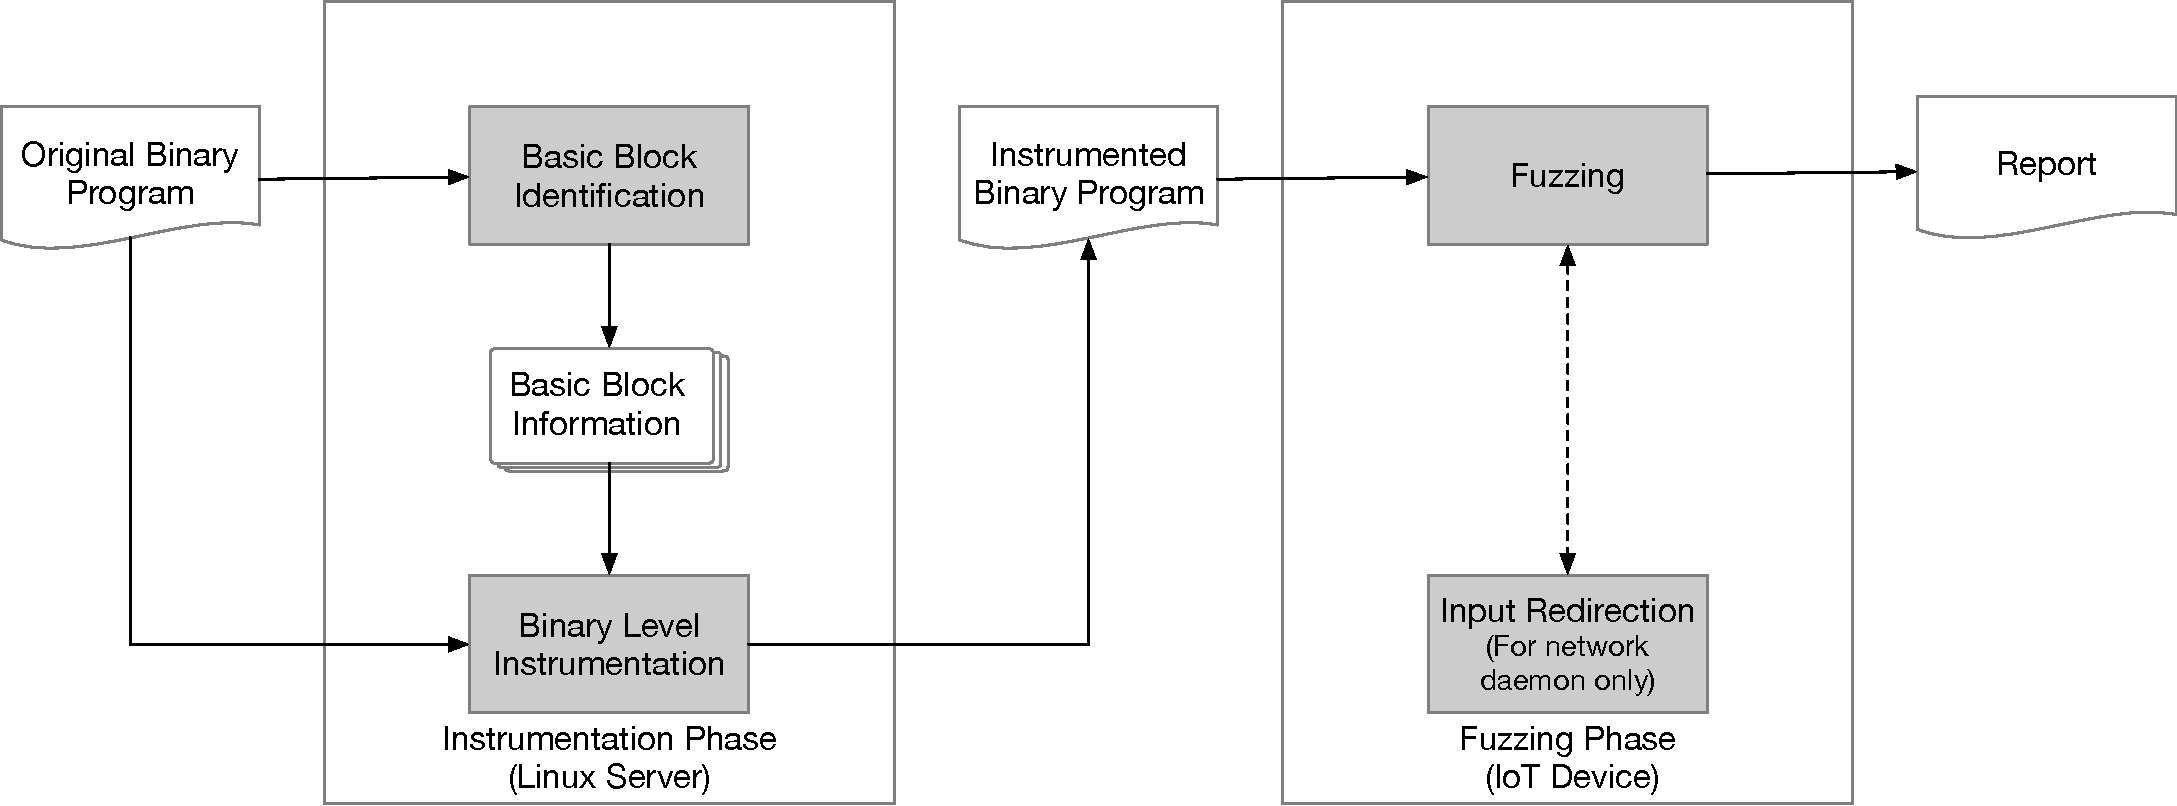
\includegraphics[width=0.9\textwidth]{arch}
\caption{ Overview of \sysname.}
\label{figs:arch}
\end{figure*}

The system overview of {\sysname} is illustrated in Figure~\ref{figs:arch}. Specifically, there are two phases in the workflow of \sysname: \textbf{instrumentation phase} and \textbf{fuzzing phase}.

In the instrumentation phase, we develop an elf-patcher and it first takes a binary program as an input, and then identifies and locates all of its basic blocks by disassembling and analyzing the binary code. Next, a small code stub for recording branch coverage is automatically instrumented into the beginning of each basic block that the elf-patcher identified. Finally, a code stub for initialization and communication with the fuzzer is automatically registered as an initialization entry of the target program. To guarantee the efficiency, all steps in the instrumentation phase are performed outside the target IoT devices. 

In the fuzzing phase, both the instrumented program and the fuzzer are deployed on the original device before an instrumentation-guided coverage-based fuzzing is performed and all the fuzzing results are recorded. Besides, IoT devices usually contains many network daemon software (e.g. a web server), so we also design and implement an input redirection framework for fuzzing on network daemons.

Overall, \sysname provides two major features: binary-level instrumentation and network input redirection. We will go through the technique details of these features in following subsections.


%[Why binary program fuzzing]?

%disassembling suffers from accuracy issues...
%Why we patch binary

% 1. The prevalence of linux-based IoT device
% 2. lack of source code 
% 3. 

%[Why coverage-based grey-box]?

%[emulator vs devices]
% 1. The limitation of emulator-based approach kernel module, 
% 2. The 




\subsection{Basic Block Identification}


The basic idea of instrumentation-guided coverage-based fuzzing is to improve execution coverage by monitoring each execution path of the target program for different inputs. To this end, each basic block of the target binary program needs to be identified with good accuracy before instrumentation. A basic block is a straight-line code sequence with no branches in except the entry and no branches out except at the exit~\cite{hennessy2011computer}. Once the execution of the target program enters a specific basic block, all code inside this basic block must be sequentially executed. 

%To ensure the accuracy of tracking execution path, a code stub which is responsible to communicate with the fuzzer needs to be instrumented into each basic block of the target program.

%Before instrumentation, it is very important to identify all the basic blocks inside the target program. %To this end, 

As illustrated in Figure~\ref{figs:arch} \sysname first leverages a static analyzer to perform reverse engineer on the target binary program including generating a hierarchical call graph and extracting a list of functions. Then for each function, \sysname checks if it can be triggered from entry point of the program by performing a backward search on the call graph. Such check eliminates those unreachable basic blocks from the results and therefore improves the efficiency of \sysname. Next, \sysname marks all reachable functions, and for each function it again leverages the static analyzer to search for all basic blocks within this function. Finally, \sysname merges the searching result, eliminates duplicated basic blocks and logs all the information (e.g. type of instruction set, base address of the basic block, size of the basic block, etc.) of each basic block for later use.

\subsection{Binary-level Instrumentation}\label{sec:design:inst}


\begin{figure}[htbp]
\centering 
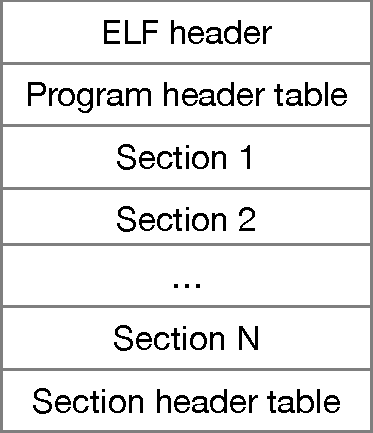
\includegraphics[width=0.2\textwidth]{elf}
\caption{Executable and Linkable Format~(ELF) File Structure.}
\label{figs:elf}
\end{figure}


\sysname targets at Executable and Linkable Format ~(ELF)~\cite{elf} binary program which is used in most Unix-like operating system. The binary-level Instrumentation that perform by \sysname is pure static and therefore only takes the target program and its basic block information as a input. 

The structure of a typical ELF file is described in Figure~\ref{figs:elf}. $ELF\ Header$ contains the basic information of the file, such as instruction set and architecture. Besides, $ELF\ Header$ also stores the position and size for both $Program\ Header\ Table$ and $Section\ Header\ Table$. $Program\ Header\ Table$ defines run-time information for the binary program. For example, $PT\_LOAD$ entries specific the mapping between sections and memory segments, $PT\_DYNAMIC$ entry specifics the position and size for $.dynamic$ section. $Section\ Header\ Table$ specifies position and size for each section within the ELF file. Such information is useful during the linking process. $Sections$ are segments where code and data are actually stored in an ELF file. There are various types of sections that defined in an ELF file, such as $.text$ section, $.data$ section, etc. Generally, $Program\ Header\ Table$ is not necessary for ELFs during linking while $Section\ Header\ Table$ is omittable for ELFs during run-time. However, most of compilers tend to keep both tables at the same time.

Our basic idea of instrumentation is to add code stub into each basic block without breaking the code logic of the original program. However, in a compiled ELF binary program, there is no space for the instrumented code in the original sections because the addresses for all the instructions and data have already been calculated by the compiler and moving such instructions or data at binary-level will likely disrupt the execution of the original program. Consequently, our solution makes extra space for instrumented code by adding new sections at the end of the ELF binary program.

As shown in Figure~\ref{figs:instrumentation}, for each basic block, we replace its first instruction $inst\_A$ with a branch instruction that redirects the program counter (PC) to a newly added section where our instrumented code is executed. Then, the replaced instruction $inst\_A$ is moved after the instrumented code. Finally, another branch instruction is added at the end of the new section to redirect PC back to the next instruction $inst\_B$ in the original section. Generally, our solution performs the following three steps for binary instrumentation:

\begin{figure}[htbp]
\centering 
\begin{subfigure}[b]{0.20\textwidth}
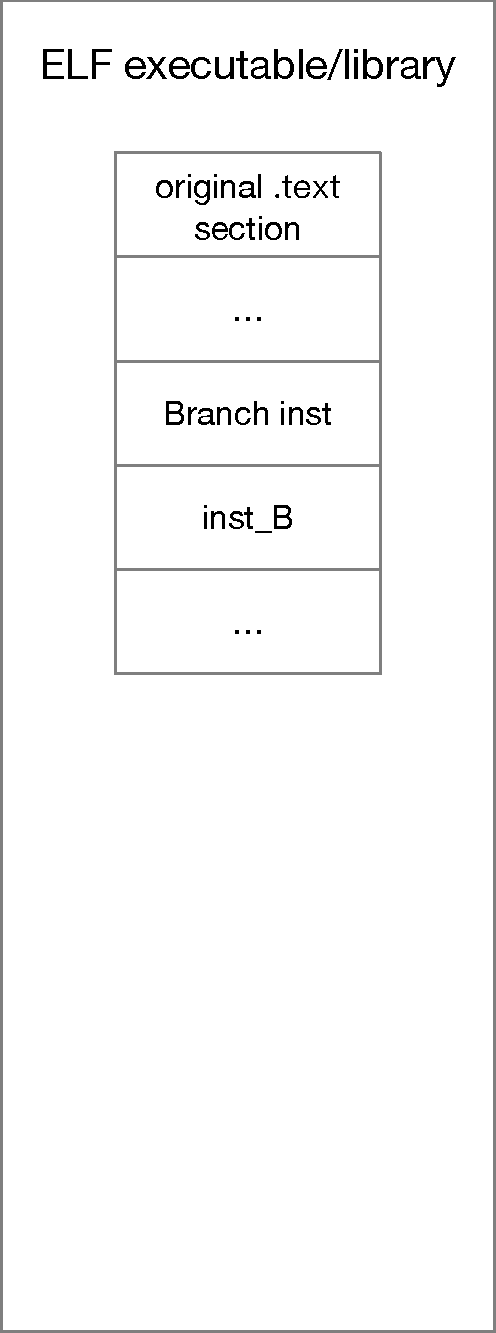
\includegraphics[width=\textwidth]{instrumentation_a}
\caption{Original ELF file}
\end{subfigure}
\hspace{+8pt}
\begin{subfigure}[b]{0.20\textwidth}
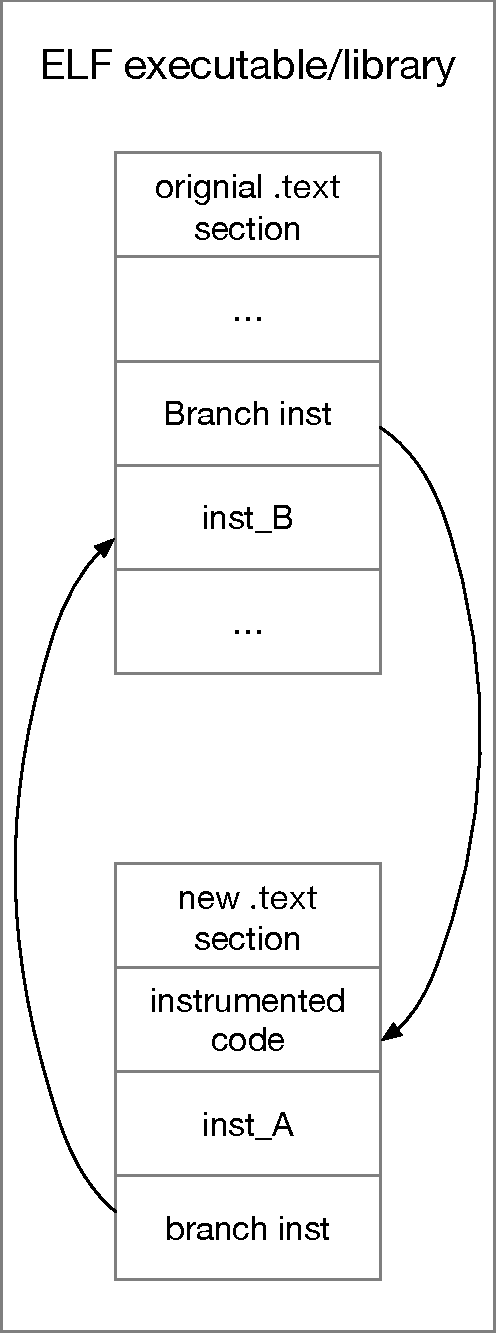
\includegraphics[width=\textwidth]{instrumentation_b}
\caption{Instrumented ELF file}
\end{subfigure}
\caption{Binary-level Instrumentation.}
\label{figs:instrumentation}
\end{figure}

\begin{enumerate}
	\item Adding new sections for instrumented code and data and updating $Section\ header\ table$ for these new sections.
	\item Adding new $PT\_LOAD$ entry in $Program\ header$ $table$ to make sure all newly added data is loaded into the memory during execution.
	\item Replacing the original instructions and adding instrumented instructions and data.
\end{enumerate}

\vspace{5pt} 
\subsubsection{\bf{Adding New Sections}}
The approach we take to add new sections in ELF binary program is quite straightforward. For new data section, we first calculate the length of the inserted data and determines the address and size of the new section. Then we add these sections directly at the end of the last section in the original program. Meanwhile, for each new data section, we will add a new entry in $Section\ header\ table$ to specify its address, offset and size. Moreover, since we expand the size of $Section\ header\ table$ which therefore increases the size of the ELF file, the ELF header also needs to be modified accordingly.

However, things are getting a little bit complicated when adding new code sections. Our code instrumentation relies on the assembler to generate new instructions. Without the size information of the newly added code section, the assembler has no idea of the section layout and relative offset from the original instructions to the inserted code stub, therefore the assembler cannot generate correct instructions for the new stub. However, the size of the new code section depends on the length of the instrumented instructions, which can only be determined by the assembler. In other words, there is a deadlock.

To solve this deadlock, our solution is to take two assemble passes. In the first pass, we assume the address for the original instructions with which the assembler is able to calculate the length of the instrumented instructions. In this way, the size of the new code section is determined and can be used in the second pass for code instrumentation.

%To solve this deadlock, our solution is to let the assembler take two passes. In the pass, we first assume the addresses for the original instructions with which the assembler is able to calculate the length of the instrumented instructions. In this way, the size of the new code section is determined and can be used in the second pass for code instrumentation. \\
\vspace{5pt} 
\subsubsection{\bf{Updating Program Header Table}}
Sections are static information in an ELF binary program. Therefore the instrumented data and instructions will not be loaded into memory by simply adding new sections to the original ELF program. We need to add $PT\_LOAD$ entries for all new sections to specify the access permission for each segment of data and the memory address where it should be loaded to.

Unlike $Section\ header\ table$ which is located at the end of the ELF file~(shown in Figure~\ref{figs:elf}), expanding $Program\ header\ table$ will inevitably erase sections that comes after it. To avoid the such conflict, we come up with two solutions: 1. Moving $Program\ header\ table$ behind all sections. 2. Moving those sections that come after $Program\ header\ table$ backwards. Unfortunately, in practice the first solution is infeasible because Linux kernel assumes that $Program\ header\ table$ comes immediately after ELF header. In other words, it will result in a failure when running the instrumented program if we moved the $Program\ header\ table$ elsewhere. We therefore adopt the second solution. We first analyze a large number of ELF binaries that we collected from dozens of IoT device firmwares. The statistics show that only certain types of section~(Table~\ref{table:elfsecs}) appears immediately after $Program\ header\ table$. All these types of sections have their location information stored in $Program\ header\ table$ or $.dynamic$ section, so they can be relocated by simply modifying the pointers accordingly. 
\begin{table}
\center
\begin{tabular}{|l|l|}
\hline 
Section & Description \\ 
\hline 
.interp & Absolute path of the loader \\ 
\hline 
.note. & Additional information about the ELF \\ 
\hline 
.hash & Symbol hash table \\ 
\hline 
.gnu.hash & GNU style symbol hash table \\ 
\hline 
.dynsym & Symbol table \\ 
\hline 
.dynstr & Strings used by .dynsym \\ 
\hline 
\end{tabular}
\caption{Types of sections that may appears after $Program\ header\ table$ in an ELF binary program.}
\label{table:elfsecs}
\end{table}

After moving all these sections, we can easily expand the $Program$ $header\ table$ by adding new entries without any conflict. For each type of the sections that we added or moved, we add a corresponding $PT\_LOAD$ entry to $Program\ header\ table$. Besides, newly added sections are granted with one of the three access permission: $READ\_ONLY$, $READ\_WRITE$ and $READ\_EXECUTE$, which is reflected in their $PT\_LOAD$ entries.
\vspace{5pt} 
\subsubsection{\bf{Wrapping Original Instruction}}\label{sec:design:wrap}

As shown in Figure~\ref{figs:instrumentation}, our code instrumentation first replaces the first instruction $inst\_A$ in each basic block of the target program with a branch instruction and thus redirect the execution to our newly added .text section. Instrumented code, the replaced $inst\_A$ and another branch instruction are then sequentially inserted into the new section.

Binary level instrumentation could be very tricky for CISC architecture~(e.g. x86), where instructions usually have variable lengths. So replacing one instruction with another may overwrite the subsequent instructions. Fortunately, most IoT devices are built upon RISC architecture~(e.g. ARM, MIPS, etc.) with fixed instruction length. As a result, $inst\_A$ can be easily replaced with a branch instruction without touching the instruction that comes after it. 

One major challenge to apply our code instrumentation is that we need to guarantee the successful execution of the original $inst\_A$~(See Figure~\ref{figs:instrumentation}) in the new location. To this end, our instrumented code maintains the values in all registers or memory addresses that are used in the original program. Specifically, our instrumented code first backs up all registers before using them and recovers those values at the end. For memory addresses, our instrumented code only writes to unused addresses below the current stack pointer to avoid potential conflicts. 

Besides, some instructions use the value of program counter~(PC). Since the value of PC varies at different position in a program, moving these PC-related instructions to new locations~(e.g. $inst\_A$ in Figure~\ref{figs:instrumentation}) may disrupt the executions of the origin program and thus result in errors. To eliminate such effect caused by PC, in our approach we first divide all instructions into the following five types based on their different relationship with PC. Then for each type, we provide a different wrap solution to the original instruction.

\begin{itemize}

\item \textbf{T1: PC-independent instruction.} These are instructions that are completely independent from the value of PC. In other words, they are not related to any computation or memory access based on the value of PC.

\item \textbf{T2: PC-dependent branch instruction.} Some branch instructions (e.g. $b$ in ARM instruction set) depend on the value of PC to determine the destination address. An offset which is relative to PC can be used as an operand to indicate the destination address.
 
\item \textbf{T3: PC read-only instruction.} These are the instructions that take the value of PC as one of their source operands, and then either assign it to another register or load a value from the memory with a relative offset to current PC.

\item \textbf{T4: PC read-only instruction with stack operation.} These instructions take the value of PC as their source operand which works just like T3 except they also involve in stack operation.

\item \textbf{T5: PC read-write instruction.} These instructions involve in both read and write operations that are related to PC.

\end{itemize}

\noindent{\bf Wrap Solution.} For each type of instruction~(T1 to T5), our approach provides a wrap solution~(S1 to S5) to eliminate the effect caused by different PC values at new positions in the target program.

\begin{itemize}

\item \textbf{S1. }~For PC-independent instruction~(T1), it will not affect their execution by moving it to a new location. As a result, no specific wrap solution is needed other than simple branch back.

\item \textbf{S2. }~For PC-dependent branch instruction~(T2), although its destination address is determined based on the value of PC, the destination address can be easily obtained by disassembling this branch instruction in the original program. In this way, the branch instruction becomes PC-independent and therefore does not require any specific wrap solution either.

\item \textbf{S3. }~For PC read-only instruction~(T3), we first find a unused register as $pivot$ and save its original value to stack. Secondly we get the value of PC at the original position of the target instruction~(e.g. $Inst\_A$ in Figure~\ref{figs:instrumentation}(a)) by using a disassembler and save it to $pivot$. Then we replace each occurrence of PC register with $pivot$ in the target instruction at new position~(e.g. $Inst\_A$ in Figure~\ref{figs:instrumentation}(b)). In the end, the value of $pivot$ register is recovered from stack after the execution of the target instruction at new position.

\item \textbf{S4. }~Compared with T3 instruction, T4 instructions involves with both the value of PC and stack operations. Thus wrap solutions in S3 may cause conflict in this situation. Empirically, T4 instructions usually push a number of registers (including PC register) to stack. So in addition to S3, we also need to coordinate the position on stack for PC, $pivot$ and other registers. The basic idea behind this wrap solution is to avoid conflict in stack memory allocation when pushing $pivot$ and PC. Our wrap solution~(S4) takes the following steps: 1. Set an unused register as $pivot$. 2. Push $pivot$ to stack for backup and load the original value of PC to $pivot$. 3. Push $pivot$ to stack again with target PC value on top the last push. 4. Recover $pivot$ from stack. 6. Push other registers. 

\item \textbf{S5. }~For PC read-write instruction~(T5), simply using S3 or S4 could lead to problems because T5 instruction sets new value to PC after execution and therefore redirects the execution of the program to somewhere else. Such redirection does not give us a chance to recover $pivot$ from stack, thus disrupts the execution of the program. To resolve these problems, we need to guarantee the recovery of $pivot$ the same time when redirect happens. Our warp solution~(S5) takes the following steps: 1. Set an unused register as $pivot$ and push $pivot$ to stack for backup. 2. Load the original value of PC to $pivot$. 3. Replace each occurrence of PC register with $pivot$ in the target instruction at new position. The destination address of redirection $RA$ will be written to $pivot$ after the execution of the target instruction. 4. Push $pivot$ to stack. 5. Pop stack twice to recover $pivot$ first and then load $RA$ to PC for redirection.
\end{itemize}

With the five wrap solutions that listed above, our approach for code instrumentation can be successfully applied in various kinds of target binary programs on many Linux-based IoT devices. Examples that demonstrate how to implement each wrap solution are given in Section~\ref{sec:impl:wrap}.
\vspace{5pt} 
%As mentioned in previous subsection, \sysname performs binary level instrumentation at the beginning of \texttt{main} function as well as the beginning of each identified basic block. Our instrumentation is pure static and therefore only takes the target program and its basic block information as a input. Generally, binary level instrumentation on programs of IoT device could be challenging for the following reasons:
%
%\begin{enumerate}
%	\item Each segment in an ELF executable is page-aligned and has limited size. So it is impossible to instrument too many instructions or data into the original segment. 
%	\item Binary level instrumentation must maintain the structure of the original program. For example, instrumented code must not affect the relative locations of original instructions, otherwise it will cause addressing problems and probably lead to a crash. 
%	\item Context switching before and after the instrumented code must be taken into careful consideration. For example, \hl{PC-related instructions?}
%	\item Some CPU architectures of IoT device may have more than one instruction set, making it more difficult to binary level instrumentation. For example, ARM CPU has two instruction set: ARM and Thumb. All instructions in ARM set are 32-bit long while those in Thumb set are mostly 16-bit long. For optimization purpose, a compiler (e.g. arm-gcc) may use instructions from both sets in different basic blocks of the same program. 	
%\end{enumerate}
%
%
%
%To address all of the above challenges, we...
\subsubsection{\bf{Library Instrumentation}}

In addition to ELF executable, shared library is another common format of Linux-based programs. Many software implements its core features in shared libraries, so it is necessary for \sysname to provide binary-level instrumentation support for shared libraries. Otherwise, our coverage-based fuzzing will not be able to track execution paths inside shared library program, which significantly reduces its efficiency and effectiveness. 

Code instrumentation on shared libraries is similar to that on ELF executables. However, there are still some challenges. For example, shared libraries are required to be compiled with position-independent code~(PIC) support\cite{pic} to achieve dynamic loading, which is usually not the case for ELF executables. With PIC support enabled, the base address of a shared library can only be determined after the library being loaded into the memory and address relocation needs to be done once the base address is determined. Such relocation process requires careful consideration during the code instrumentation.

Next, we describe how to address these two challenges in our approach.
\vspace{5pt} 

\noindent{\bf Fuzzing Initialization.} A coverage-based fuzzer usually requires to instrument a piece of code at the beginning of the target program for initialization purpose. In our approach, we leverage on $.init\_array$ section in an ELF file to execute initialization code in the target program. $.init\_array$ is an array where each element specifies a function to be executed at the beginning of the execution. As a result, by instrumenting new elements into $.init\_array$, we can successfully execute fuzzing initialization code in a shared library.
\vspace{5pt} 

\noindent{\bf Relocation.} Code instrumentation on a target binary that compiled with PIC support inevitably needs additional work of relocation. Specifically, we need to take relocation into consideration in the following three situations: 1. Moving or modifying any original data sections. 2. Instrumenting code into the original code sections. 3 Instrumenting code or data into the newly added sections. 

As to the first situation, since $.init\_array$ is the only original data section that we move or modify in our code instrumentation, we only need to perform relocation for every new element that we add into $.init\_array$ section.

For the second situation, if our code instrumentation replaces original instructions with new instructions, we simply need to delete the previous relocation and performs new relocation for the newly added instructions. 

For the last situation, we first record all the symbols that occur during instrumentation, find locations where these symbols are referenced by comparing each piece of instrumented code and then perform relocation for each symbol in the order of occurrence.

After resolving the relocation issue, the instrumented shared library can be used to track path information during our coverage-based fuzzing process, which obviously increases the efficiency and accuracy of \sysname.

\subsection{Fuzzing on Network Daemons}\label{sec:design:daemons}

Most of fuzzers target at programs that take input from a local file~(e.g. a parser program) or standard I/O streams~(e.g. a command-line program). In coverage-based fuzzing, this input is constantly changed by the fuzzer according to the coverage information that it collected during the execution of the target program. However, things are completely different on IoT devices. Since IoT devices are ideally designed to fulfil the connectivity of different ``things'', network servers or daemons have become the most dominant type of software on IoT devices. Instead of reading input from file or standard I/O streams, network daemons listen on certain ports and interact with clients from other devices. So the major challenge to fuzz on network daemons is to find an approach for efficient input redirection. 

The first approach that can be easily think of is to set up a transparent proxy, which acts as a client for the target network daemon. Whenever the fuzzer starts, instrumented code stub inside the target daemon is first triggered and the proxy is then notified to send new input that generated by fuzzer. As one its advantages, this approach does not require any modification to the code logic of the original network daemon, so it is easy to implement and deploy. However, network operation is too expensive to be involved in fuzzing. For example, the latency for a network daemon to bind on a certain port is usually several milliseconds on Linux-based IoT devices, which is apparently unacceptable in fuzzing. Consequently, a proxy-based approach is infeasible.

Since the major overhead comes from network operation and such operations are usually manipulated by socket APIs, our approach performs an efficient input direction by hooking socket APIs to map input from standard I/O stream to network sockets. In this way, expensive network operations at OS level are successfully avoided and the efficiency of input redirection is tremendously improved. In our approach, we first specify a port number $target\_port$ before fuzzing starts and therefore all the operations of the target daemon program on this port will be mapped to standard I/O stream accordingly. The reason to specify $target\_port$ is to avoid conflict that caused by the target daemon program listening on multiple ports simultaneously. Secondly, we hook $bind()$ API to check if it is going to bind on $target\_port$. If so, an unnamed pair of connected sockets are then created by $socketpair()$ API to act as a full duplex pipe for input/output redirection. Specifically, in our approach we hook the following three types of socket APIs:

\begin{enumerate}
\item Basic socket APIs~(e.g. $socket()$, $bind()$, $listen()$, $accept()$ and $close()$).
\item Socket APIs that specify file descriptors to listen on in user-space~(e.g. $select()$ and $poll()$). 
\item Socket APIs that register file descriptors to listen on in kernel-space~(e.g. $epoll\_create()$, $epoll\_ctl()$ and $epoll\_wait()$).
\end{enumerate}

Next, we illustrate the detailed hook operations when each of the following socket APIs is called in the target daemon program.

\begin{itemize}
\item {\bf socket()} The $socket()$ API is used to create socket file descriptor. For a newly created socket file descriptor, we have no idea if it is our target socket for input redirection until it is bind to a certain port. So here we only label this file descriptor for later use.

\item {\bf bind()} At this point, port number is already specified by parameters. If it matches $target\_port$, we mark its file descriptor as $bind\_fd$ and return success immediately. Otherwise, call the original $bind()$ API.

\item {\bf listen()} Return success immediately if the socket file descriptor matches $bind\_fd$. Otherwise, call the original $listen()$ API.

\item {\bf accept()} If the socket file descriptor does not matches $bind\_fd$, call the original $accept()$ API. Otherwise, create a socketpair~(as a pipe) of the same type with $bind\_fd$ and mark the two ends of the pipe as $A$ and $B$. Then create two threads to redirect from $stdin$ to $B$ and $B$ to $stdout$ respectively. Finally return $A$ as $accept\_fd$.

\item {\bf close()} If the socket file descriptor does not matches $bind\_fd$, call the original $close()$ API. Otherwise, exit the target daemon program immediately and notify the fuzzer to start the next instance.

\end{itemize}

In general, hooking the basic socket APIs that listed above would be sufficient to fuzz on most network daemon programs except for those listening on a list of file descriptors asynchronously. To make our approach more complete, we also hook the following two APIs:


\begin{itemize}
\item {\bf select()/poll()} $select()$/$poll()$ is used specify a list of socket file descriptors to listen on. As mentioned previously, we return success immediately without actually binding $bind\_fd$ to a certain port. So we will never get notification on $bind\_fd$ even if $bind\_fd$ is in the file descriptor list of $select()$/$poll()$ API. As a result, we simply remove $bind\_fd$ from the list and then call the original $select()$/$poll()$ API. Finally, we manually add event notification for $bind\_fd$ on return.

\item {\bf epoll} $epoll$ is another set of socket APIs that are used to listen on multiple file descriptors asynchronously. The major difference is that the file descriptor list that created by $epoll$ is maintained in kernel-space. We take similar operation as in $select()$/$poll()$ to remove $bind\_fd$ from the list before calling to original $epoll$ API. In addition, $epoll$ allows the program to attach a 64-bit long data to each file descriptor, so we need to record all the operations on $epoll$ to provide correct information for $bind\_fd$ on return.

\end{itemize}
%\subsection{Fuzzer Integration}
\section{Implementation}\label{sec:impl}
%IDA ARM platform
In this section, we describe technical details as well as challenges to implement~\sysname. 

\subsection{Fuzzer integration}\label{sec:impl:integ}
Recall that our goal is to perform efficient coverage-based guided fuzzing on binary programs in Linux-based IoT devices. To this end, our work is mainly focused on
how fuzzer interacts with the target binary program instead of improving its fuzzing strategies. As a result, we adopted AFL directly into our fuzzing framework, leverage on instrumented code to track branch coverage information and make it fully compatible to work with AFL. This also guarantee that any improvement from AFL community will also benefits our system without any modifications. Beside, we compiled the AFL initialization code into a shared library, so it can be loaded into target program before the initialization phase of fuzzing, and then the fork-server and shared memory in AFL will be initialized by the code stub that we instrument into the target program via specific interfaces in the shared library.

\subsection{Device Setup}

As mentioned in previous sections, hardware resources are extremely limited on the most of IoT devices, where most vendors will deploy a streamlined runtime library such as $uClibc$ instead of standard C library $libc$, causing problems when fuzzing on these devices. AFL requires certain symbols in $libc$ to execute correctly. However, such symbols are sometimes missing on the IoT devices where $uClibc$~\cite{uclibc} is deployed. Our solution is to performs static compilation specifically for each device, so additional library dependencies are unnecessary.  

Besides, the ELF loader that comes with some IoT devices does not enable TLS (Thread local storage)-related support. Therefore programs with TLS variables cannot be loaded on these devices. AFL requires TLS support to track the execution path of different thread in the target program. Fortunately, we notice that even though sometimes the ELF loader may not provide TLS support, however, the Linux kernel is compiled with TLS feature enabled. Thus we can easily fix the problem by just rebuilding a new version of ELF loader with TLS support enabled for the target IoT device and switch to this new loader when necessary.

In addition, most COTS IoT devices do not preserve debug interfaces for shell access, which is a basic requirement for fuzzing on device. Fortunately, such debug interfaces do exist in most devices for factory testing. For security reasons, these interfaces are usually blocked after passing all tests. So we use several tricks to activate these debug interface in order to enable shell access.

\subsection{Basic Block Identification}
Most binaries from IoT devices are stripped, which can be challenging for reverse engineering tools to completely identify the code that resides in the binary. But as we mentioned in previous sections, a failure in identifying certain basic blocks will only affect path resolution accuracy in AFL and does not cause any error in fuzzing. We test several existing opensource reverse engineering tools, such as Barf~\cite{heitman2014barf}, Sibyl~\cite{sibyl} and Miasm\cite{miasm}, but none of them could provide acceptable accuracy. So we end up leveraging on IDA Pro~\cite{ida}, a well-known commercial reverse engineering tool. It retrieves basic blocks information from the target binary program with good accuracy which meets the requirement of binary level instrumentation.


\begin{figure*}[htbp]
\centering
\begin{subfigure}[b]{0.48\textwidth}
\begin{lstlisting}[language=ARMASM,label=lst:s3_1, firstnumber=1][htbp]
loc_1000: add r1, pc, r2
loc_1004: ...
loc_1008: ...
...
...
\end{lstlisting}
\caption{Original Code}
\end{subfigure}%
\begin{subfigure}[b]{0.48\textwidth}
\begin{lstlisting}[language=ARMASM,label=lst:s3_2, firstnumber=1][htbp]
stmdb sp, {r3}
ldr r3, =loc_1008
add r1, r3, r2
ldmdb sp, {r3}
b loc_1004
\end{lstlisting}
\caption{After Instrumentation}
\end{subfigure}%

\caption{Wrap Solution for T3 instructions~(ARM).}
\label{figs:t3}
\end{figure*}


\begin{figure*}[htbp]
\centering
\begin{subfigure}[b]{0.48\textwidth}
\begin{lstlisting}[language=ARMASM,label=lst:s4_1, firstnumber=1][htbp]
loc_1000: push {r0, r2, r4, pc}
loc_1004: ...
loc_1008: ...
...
...
...
...
\end{lstlisting}
\caption{Original Code}
\end{subfigure}%
\begin{subfigure}[b]{0.48\textwidth}
\begin{lstlisting}[language=ARMASM,label=lst:s4_2, firstnumber=1][htbp]
sub sp, sp, 4
stmdb sp, {r1}
ldr pivot, =loc_1008
stmia sp, {r1}
ldmdb sp, {r1}
push {r0, r2, r4}
b loc_1004
\end{lstlisting}
\caption{After Instrumentation}
\end{subfigure}%

\caption{Wrap Solution for T4 instructions~(ARM).}
\label{figs:t4}
\end{figure*}




\begin{figure*}[htbp]
\centering
\begin{subfigure}[b]{0.48\textwidth}
\begin{lstlisting}[language=ARMASM,label=lst:s5_1, firstnumber=1][htbp]
loc_1000: ldr pc, [pc, r3, lsl#2]
loc_1004: ...
loc_1008: ...
...
...
...
...
\end{lstlisting}
\caption{Original Code}
\end{subfigure}%
\begin{subfigure}[b]{0.48\textwidth}
\begin{lstlisting}[language=ARMASM,label=lst:s5_2, firstnumber=1][htbp]
sub sp, sp, 4
stmdb sp, {r1}
add sp, sp, 4
ldr pivot, =loc_1008
ldr r1, [r1, r3, lsl#2]
stmdb sp, {r1}
ldmdb sp, {r1, pc}
\end{lstlisting}
\caption{After Instrumentation}
\end{subfigure}%

\caption{Wrap Solution for T5 instructions~(ARM).}
\label{figs:t5}
\end{figure*}

\subsection{Instruction Wrapping}\label{sec:impl:wrap}

%As mentioned in Section~\ref{sec:design:wrap}, to guarantee successful execution of the original instruction~(e.g. $inst\_A$ in Figure~\ref{figs:instrumentation}) at new position, we provide different wrap solutions for various types of instructions. In this section, we demonstrate how we implement these solutions on ARM platform. Our current implementation of \sysname only targets at binary programs in ARM devices. 

As mentioned in Section~\ref{sec:design:wrap}, to guarantee successful execution of the original instruction~(e.g. $inst\_A$ in Figure~\ref{figs:instrumentation}) at new position, we provide different wrap solutions for various types of instructions in binary level instrumentation. We successfully apply all these solutions~(Section~\ref{sec:impl:wrap} S1-S5) in \sysname for ARM binary programs. Although our current implementation of \sysname only targets at binary programs on ARM platform, these wrap solutions are general and can be ported to binaries on other platforms~(e.g. MIPS) without much effort. Next, we give examples to demonstrate how we implement these wrap solutions, specifically S3, S4 and S5 for T3,T4 and T5 instructions. We omit T1 and T2 instruction here because their wrap solutions~(S1 and S2) are relatively simple to understand.

For PC-read-only instruction~(T3),  it reads from PC but writes somewhere else. For example, $add r1, pc, r2$ is a typical T3 instruction on ARM platform. As we described in S3, first we need to find a unused pivot register, save its original value to stack, and store the value of PC. Here we choose $r3$ as a pivot register and the wrap solution for $add r1, pc, r2$ is illustrated in Figure~\ref{figs:t3}.

For PC read-only instruction with stack operation~(T4), it acts just like T3 instructions except involving stack operation. As a result, we need to coordinate the position stack for PC, pivot register and other registers. For example, $push {r0, r2, r4, pc}$ is a typical T4 instruction on ARM platform. If we choose  $r1$ as a
pivot register, then the wrap solution for $push {r0, r2, r4, pc}$ is illustrated in Figure~\ref{figs:t4}.

For PC read-write instruction~(T5), it involves in both read and write operations that are related to PC. Figure~\ref{figs:t5} demonstrates how we implement S5 for a typical T5 instruction $ldr pc, [pc, r3, lsl\#2]$ where $r1$ is chosen as the pivot register.


We implemented our binary level instrumentation framework for ELF binaries by leveraging on keystone-engine~\cite{keystone} as an assembler and capstone-engine~\cite{capstone} as a disassembler. Both of them support a variety of architectures, making it possible for our system to easily adapted to binary programs from other architectures. Overall, our binary level instrumentation framework is implemented in python with 5300 lines of code.


\subsection{Input Redirection}
For network daemon programs, we implement an efficient input redirection mechanism between a fuzzer and a target network daemon programs. Specifically, we implement a shared library called $libsockets$ in which we rewrite all of the common Linux socket APIs~(See Section~\ref{sec:design:daemons}). With dynamic linking, we successfully hook all these socket APIs in the execution of the network daemon programs using $libsockets$ and performs checks on parameters to determine whether to intercept or forward network traffic.  In total, the implementation of input redirection takes about 300 lines of python code and 3000 lines of C code.

% toolchain and compilation
%TLS support

%\section{Device Setup}
\section{Evaluation}\label{sec:eval}


In this section, we evaluate \sysname on both benchmarks and real-world IoT devices in terms of its correctness, performance and effectiveness.

%First, we evaluate \sysname on 4 GNU core utilities programs from LAVA-M dataset to see if \sysname can indeed find bugs inside programs. 

%Then, we use the same 4 programs to evaluate its performance by running both \sysname instrumented binaries and AFL compiled binaries for each of the program with a fixed amount of time. To minimize the randomness AFL introduces, each program was evaluated several times. 


\subsection{Evaluation on Benchmarks}

As mentioned in previous sections, \sysname allows coverage-based fuzzers~(e.g. AFL) to run on Linux-based IoT devices by implementing binary level instrumentation. Although our approach does not involve any modification to fuzzing strategy of the original fuzzer, we leverage a well-known fuzzer benchmark: LAVA-M~\cite{dolan2016lava} to evaluate its correctness and performance. 

\subsubsection{Correctness}
To verify the correctness of our approach, we need to run \sysname on a dataset with ground-truth to see if it can correctly fuzz a program and find bugs. LAVA-M is a widely-used fuzzer benchmark that automatically injects a large number of bugs into four GNU core utilities programs: $uniq$, $base64$, $who$ and $md5sum$. We selected the $uniq$ program to compare AFL and \sysname. Since AFL cannot run on real device, we ran this experiment on Ubuntu 16.04 in the QEMU-ARM emulator, where each host is configured with 2 cores and 4GB memory. 

% However, existing research~\cite{chen2018angora} shows that AFL does not perform well on all these four programs in LAVA-M dataset and it can only find certain number of bugs within program uniq and almost none within others. Given that \sysname simply integrates AFL to generate input and does not optimize AFL’s fuzzing strategy, we certainly cannot expect it to find more bugs than AFL. 

We ran two experiments on $uniq$ program in parallel, one using AFL and the other using \sysname. To mitigate the impact of randomization during fuzzing, we repeated each experiment six times. In the experiment with AFL, we first compiled the $uniq$ program from the source code with afl-clang-fast and then ran it with AFL on a single core for 10 hours. AFL performs a LLVM level instrumentation during compilation. In comparison, our \sysname experiment performed binary level instrumentation on a pre-compiled version of $uniq$ program. We compiled it using the same source code and parameters of afl-clang-fast as in the AFL experiment. Similarly, the experiment lasted for 10 hours on a single core.

We used several metrics provided by AFL to measure the fuzzing process. First, the number of unique crashes indicates the identified bugs. Second, the branch coverage indicates the proportion of branches that were executed in the fuzzing process. Third, the number of total path reflects the number of unique execution paths triggered by fuzzer. Table~\ref{table:res_comp} shows that the \sysname and AFL experiments have similar results, which demonstrates the correctness of \sysname.

%We first compile the uniq program with afl-clang-fast, which comes with AFL, and then run AFL for about 10 hours on a single core. In order to eliminate the impact of AFL's random mutation, we repeat the experiment three times to get the following results. The first experiment triggered 6 unique crashes, and the third triggered 4. The detailed results are illustrated in Table~\ref{table:res_afl}.

%In comparison, we use clang to compile uniq with the same parameters as afl-clang-fast and then instrument the target binary with \sysname. We test instrumented program for a total of 6 times, giving each fuzz instance about 10 hours of running time on a single core. In 6 sets of tests~(See Table~\ref{table:res_ours}), we can find crashes every time, and up to 6 unique Crashes can be triggered. The results of the test, including bitmap coverage and total paths found, are basically the same as those of the AFL compiled program. This result proves the correctness of \sysname, which is quite the same as AFL with source code.

%In other work (Angora), AFL found 9 unique crashes in uniq when the single core was running for 5 hours. Although the result in our experiment is not as good as theirs but noticed that we are running under emulation, which is much slower than a real x86 environment.


\begin{table}
\scriptsize
\renewcommand\arraystretch{1.2}
\center
\begin{threeparttable}
\begin{tabular}
{
|C{0.05\textwidth}
|C{0.045\textwidth}
|C{0.045\textwidth}
|C{0.055\textwidth}
|C{0.03\textwidth}
|C{0.05\textwidth}
|
}
%\toprule
\hline
\rmfamily\textbf{Tool}&
\rmfamily\textbf{\# of Run}&
\rmfamily\textbf{\# of Unique Crash}&
\rmfamily\textbf{Branch Coverage}&
\rmfamily\textbf{\# of Total Path} &
\rmfamily\textbf{Execution Time~(H)}
\\
%\midrule
\hline
\multirow{6}*{AFL} &
1 & 6 & 29.82\% & 75 & 10 \\
\cline{2-6}
~& 2 & 0 & 29.82\% & 80 & 10 \\
\cline{2-6}
~&3 & 4 & 29.82\% & 77 & 10 \\
\cline{2-6}
~&4 & 0 & 29.82\% & 78 & 10 \\
\cline{2-6}
~&5 & 4 & 29.82\% & 83 & 10 \\
\cline{2-6}
~&6 & 4 & 29.82\% & 71 & 10 \\
\hline

\multirow{6}*{\sysname} &
1 & 6 & 29.64\% & 79 & 10 \\
\cline{2-6}
~ & 2 & 1 & 29.64\% & 76 & 10 \\
\cline{2-6}
~ &3 & 1 & 29.64\% & 74 & 10 \\
\cline{2-6}
~ &4 & 4 & 29.64\% & 82 & 10 \\
\cline{2-6}
~ &5 & 3 & 29.64\% & 76 & 10 \\
\cline{2-6}
~ &6 & 1 & 29.64\% & 78 & 10 \\
\hline
\end{tabular}

%\footnotesize
%\item[1] APIs of embedded ad are found in both in Java code~(299 APIs) and XML~(108 APIs) layout resource files in apps~(Listing~\ref{lst:bannerlayout1} and Listing~\ref{lst:bannerlayout2}).
%\end{tablenotes}
\end{threeparttable}
\caption{\label{table:res_comp}Fuzzing Test Result on $uniq$ in Lava-M Dataset with AFL and \sysname.}
\end{table}

% \begin{table}
% %\ttfamily
% \scriptsize
% \renewcommand\arraystretch{1.2}
% \center
% \begin{threeparttable}
% \begin{tabular}
% {
% |C{0.05\textwidth}
% |C{0.05\textwidth}
% |C{0.1\textwidth}
% |C{0.05\textwidth}
% |C{0.1\textwidth}
% |
% }
% %\toprule
% \hline
% \rmfamily\textbf{Number of Run}&
% \rmfamily\textbf{Unique Crashes}&
% \rmfamily\textbf{Bitmap Coverage}&
% \rmfamily\textbf{Total Paths} &
% \rmfamily\textbf{Execution Time~(H)}
% \\
% %\midrule
% \hline
% 1 & 6 & 0.44\% & 79 & 10 \\
% \hline
% 2 & 1 & 0.44\% & 76 & 10 \\
% \hline
% 3 & 1 & 0.44\% & 74 & 10 \\
% \hline
% 4 & 4 & 0.44\% & 82 & 10 \\
% \hline
% 5 & 3 & 0.44\% & 76 & 10 \\
% \hline
% 6 & 1 & 0.44\% & 78 & 10 \\
% \hline
% \end{tabular}
% %\footnotesize
% %\item[1] APIs of embedded ad are found in both in Java code~(299 APIs) and XML~(108 APIs) layout resource files in apps~(Listing~\ref{lst:bannerlayout1} and Listing~\ref{lst:bannerlayout2}).
% %\end{tablenotes}
% \end{threeparttable}
% \caption{\label{table:res_ours}Fuzzing Test Result on $uniq$ in Lava-M Dataset with \sysname.}
% \end{table}


\begin{figure}[htbp]
\centering

\begin{subfigure}[b]{0.48\textwidth}
       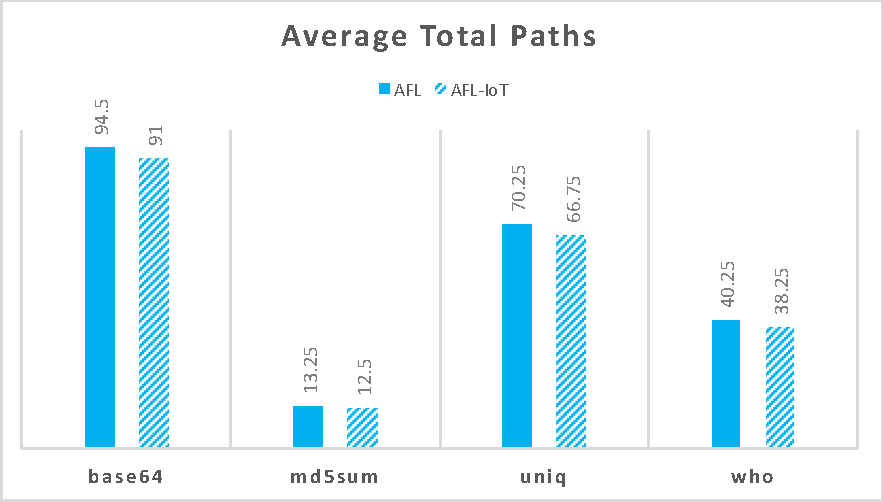
\includegraphics[width=\textwidth]{paths}
        \caption{Average Total Paths}
    \end{subfigure}%
\vspace{5pt}
%\begin{subfigure}[b]{0.48\textwidth}
%        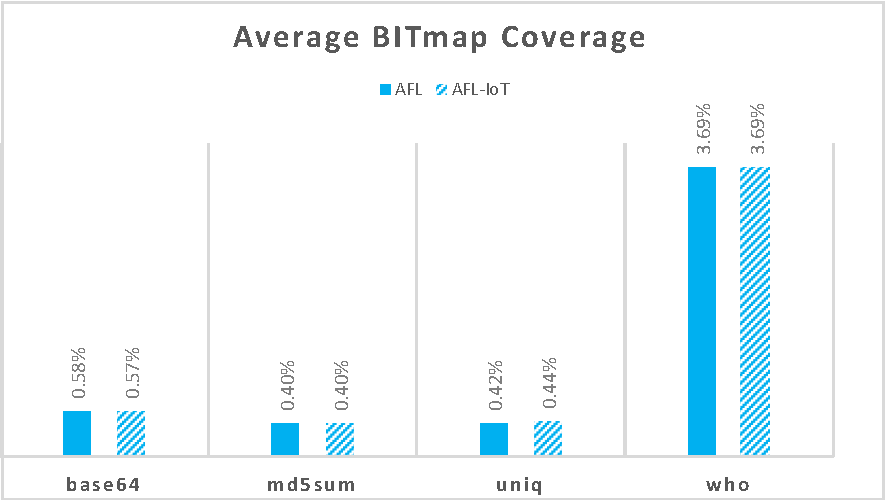
\includegraphics[width=\textwidth]{coverage}
%        \caption{Average Bitmap Coverage}
%    \end{subfigure}%
%\vspace{5pt}
\begin{subfigure}[b]{0.48\textwidth}
        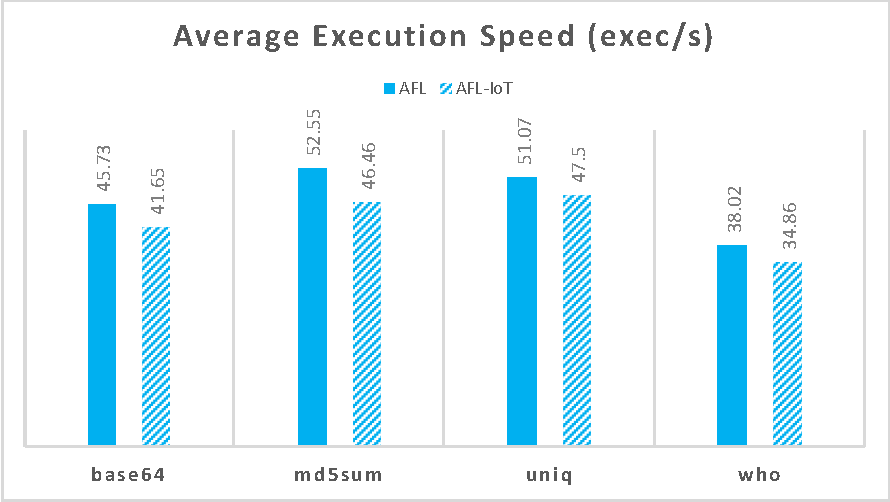
\includegraphics[width=\textwidth]{execspeed}
        \caption{Average Execution Speed}
    \end{subfigure}%

\caption{Performance Comparison Between AFL and \sysname.}
\label{figs:performance}
\end{figure}

\subsubsection{Performance}\label{sec:eval:performance}

In addition to correctness, performance is also vital for fuzzing. Since \sysname performs binary level instrumentation on target programs, it lacks source code level information, making instrumented code optimization even impossible. As a result, programs that instrumented at the binary level inevitably suffer from performance overhead in comparison with those with source code instrumentation. To evaluate \sysname, we compared the fuzzing test performance between source code level instrumentation by AFL and binary level instrumentation by \sysname. We again chose the LAVA-M dataset. This time we tested AFL and \sysname on all the four programs in LAVA-M with the same experiment environment as in our previous evaluation: dual-core CPU with 4GB memory under QEMU-ARM emulator. Similarly, for each target program, we built two versions: one compiled from source code with afl-clang and then run with AFL, another compiled with clang using the same parameters and then run with \sysname after binary level instrumentation. To mitigate the influence of randomness, we ran each version of the four program four times. The test of each running instance lasted for one hour on a single core.

We chose the number of total paths and execution speed as indicators of performance. Figure~\ref{figs:performance} compares the performance between AFL and \sysname. For all the four target programs, there is a 5\% average decrease for \sysname with instrumented programs in comparison with AFL with compiled programs in terms of number of total paths. The main reason of this decrease is that the instrumented programs ran slower than the compiled ones, resulting in a decrease in the number of instances that the fuzzer can execute in the same time. This affects the number of input that the fuzzer can mutate and therefore reduces the number of total paths.

%the version that instrumented by \sysname and the version AFL compiled from source code are almost consistent in terms of bitmap coverage.


%Recall that our instrumented version even gets a higher bitmap coverage In the $uniq$ test

%In the $uniq$ test, our instrumented version even gets a higher bitmap coverage. It should be noted that because \sysname uses the disassembler to locate basic blocks within the program, the result obtained is different from the what clang gets. Therefore, the ”bits” in the bitmap are not exactly the same of these two, it can only be a rough estimate of the coverage. 

Among all four programs in LAVA-M dataset, the instrumented versions have an execution speed drop of about 10\% on average compared with the compiled versions. This performance overhead can be attributed to the following three reasons:

\begin{enumerate}
    \item As \sysname performs instrumentation at binary level, it does not have enough context information, which makes it impossible to optimize the instrumented code stub. Therefore, \sysname must save all used registers every time when it enters the instrumented code stub. In contrast, AFL's source-based instrumentation can take full advantage of the compiler's optimization capabilities to avoid saving context frequently. Besides, it can also use idle registers to store data such as pointers globally, thus yielding a faster execution of instrumented code stubs.
    
    \item As mentioned in the design and implementation sections, we need to wrap the original instruction at the target address during the binary level instrumentation to ensure that the overwritten instruction can be executed as expected in the instrumented code segment. This inevitably introduces pivot-related operations together with expensive memory access instructions, which will slow down the execution of the target program.
    
    \item Finally, to guarantee the integrity of the original program, we place the instrumented code and data at the end of the entire program. 
    When loaded into the memory for execution, the program needs to jump to the instrumented code frequently to record the execution path. Since the original code segment of the program is far away from the instrumented code segment in memory, they cannot be loaded into the CPU cache at the same time. This frequent back and forth jump can cause a large number of instruction cache misses, which further adds additional overhead to the execution of the program.
\end{enumerate}

Overall, compared with AFL, \sysname achieves the similar code coverage performance, only about 5\% decrease in average number of total path and about 10\% decrease in average execution speed on binary programs. With slight performance overhead, \sysname is fully capable of fuzzing binary programs on most Linux-based IoT devices, where resources are very limited.

\subsection{Evaluation on Real-world IoT devices}\label{sec:eval:real}

The ultimate goal of \sysname is to fuzz binary programs in COTS Linux-based IoT devices. Since we have evaluated \sysname on benchmarks for its correctness and performance, next we can evaluate it on real-world IoT devices. Our evaluation selects 4 popular ARM Linux-based home routers from three well-known device manufacturer: ASUS AC1700, Xiaomi R1D/R3D and Netgear R7000. 


%Considering the popularity and the computational power, we pick three real-world COTS smart router, which are ASUS AC1700, Xiaomi R1D and Netgear R7000, as the target devices of our evaluation.

We upgraded all the four devices to the latest version of firmware and got shell access on each device using the debugging interfaces. Next, we selected dozens of command-line programs and daemon programs from each device. We determined how to interact with these programs and where to feed input to them by analyzing their behaviors. Since these programs are designed to run on these devices, they can be executed directly without further environment configuration or dependency resolution. For programs that read from the standard input or from a file, we performed binary level code instrumentation with with \sysname directly. For those designed to read input from network~(e.g. daemon programs), we additionally applied our approach described in Section~\ref{sec:design:daemons} to redirect the input to specific network interfaces and ports. Overall, our evaluation performed binary level instrumentation and fuzzing on over 100 binary programs on the four devices. For each fuzzing instance, we used a single-core CPU and ran within 24 hours.

\begin{table*}[htpb]
%\ttfamily
\scriptsize
\renewcommand\arraystretch{1.2}
\center
\begin{threeparttable}
\begin{tabular}
{
|C{0.05\textwidth}
|C{0.1\textwidth}
|C{0.1\textwidth}
|C{0.1\textwidth}
|C{0.06\textwidth}
|C{0.06\textwidth}
|C{0.06\textwidth}
|C{0.1\textwidth}
|C{0.1\textwidth}
|
}
%\toprule
\hline
\rmfamily\textbf{No.}&
\rmfamily\textbf{Binary Program}&
\rmfamily\textbf{Program Type}&
\rmfamily\textbf{Device}&
\rmfamily\textbf{Execution Time~(H)}&
\rmfamily\textbf{Branch Coverage}&
\rmfamily\textbf{Total Paths} &
\rmfamily\textbf{Execution Speed~(exec/s)} &
\rmfamily\textbf{Unique Crashes}
\\

\hline
1&	bunzip2\tnote{1}&   command-line&    Xiaomi R1D      &14&	2.27\%&	 203&	82  &	    11\\\hline
2&	bzcat\tnote{1}&	    command-line&    Xiaomi R1D      &12&	2.27\%&	 202&	111  &      13\\\hline
3&	gunzip\tnote{1}&	command-line&    ASUS AC1700             &14&	3.19\%&	 204&	35 &	    20\\\hline
4&	gzip\tnote{1}&	    command-line&    Netgear R7000            &12&	3.38\%&	 255&	124 &	    30\\\hline
5&	lzcat\tnote{1}&	    command-line&    Xiaomi R1D      &14&	0.96\%&	 78&	76&	        1\\\hline
6&	unlzma\tnote{1}&	command-line&    Xiaomi R1D      &12&	1.00\%&	 79&	94&	        4\\\hline
7&	zcat\tnote{1}&	    command-line&    Netgear R7000             &12&	3.23\%&	 224&	103&	    30\\\hline
8&	unzip&	            command-line&    ASUS AC1700              &12&	45.57\%&	 626&	278&	    12\\\hline
9&	tsar&	            command-line&    Xiaomi R1D      &14&	22.82\%&	 45&	22&	        14\\ \hline
10&	plugincenter&       network daemon & Xiaomi R1D  &14&	11.32\%&	262&	16&	        22\\\hline


\hline
\end{tabular}
\begin{tablenotes}
\footnotesize
\item[1] These programs are common Linux utilities that are integrated into a single executable called Busybox~\cite{busybox}. Since it combines many different programs in one executable, the branch coverage for each of them is relatively low.
\end{tablenotes}
\end{threeparttable}
\caption{\label{table:res_iot}Fuzzing Test Result in Real-world COTS Linux-based IoT Devices with \sysname.}
\end{table*}


Table~\ref{table:res_iot} shows the crashes that \sysname found in 10 different binary programs. The first seven programs are archive tools included in Busybox, a popular Linux utility toolbox for IoT devices. \sysname found as many as 30 unique crashes in these programs. Further analysis shows that most of the bugs have been fixed in the latest version of Busybox. Notably, one crash from lzcat and two crashes of unlzma were fixed just a few months before our evaluation, which demonstrates \sysname's ability to find real software bugs. In addition to the bugs in Busybox, \sysname also found 12 unique crashes in the independent archive program unzip. The ninth program in Table~\ref{table:res_iot} is a third-party version of sar~(System Activity Reporter)~\cite{sar}, in which \sysname found 14 unique crashes. The last one, plugincenter, is a daemon program from Xiaomi R1D smart router. Although daemon programs generally needs to do a series of initialization when starting, which could slow down the execution speed, \sysname still found 22 unique crashes in it.

In summary, \sysname is a fast, lightweight and easily deployable coverage-based fuzzing framework for binary programs on Linux-based IoT device. The major advantage of \sysname over other fuzzers is that it directly instruments the target program at the binary level, which makes it possible to fuzz various types of IoT devices with slight performance overhead. Our evaluation shows that \sysname is accurate and effective in finding bugs in binary programs on real world Linux-based IoT devices, and it only has about 10\% runtime overhead in comparison with AFL.
\section{Limitation}\label{sec:limit}
Although \sysname has been proved as an lightweight fuzzing tool for Linux-based IoT devices with good efficiency and accuracy, we still acknowledge the following limitations:
\begin{itemize}

 \item {\bf Accuracy of binary level instrumentation.} As described in previous sections, \sysname first leverage IDA Pro~\cite{ida} to identify all basic blocks in the target binary program and then for each basic block it performs binary level instrumentation. As a reverse engineer tool, IDA Pro usually achieves good accuracy. However, it is still possible for it to miss a small number of basic blocks in the target program, which can eventually affect the accuracy of binary level instrumentation in our approach. Empirically, IDA Pro can miss up to 5\% of basic blocks. Please note that such inaccuracy will only result in loss of branch coverage information in fuzzing process and will not affect the correctness of program execution.   
 
 \item {\bf Efficiency of fuzzing on network daemon.} For network daemon programs, \sysname performs input redirection by hooking socket APIs. Although such feature has eliminated major performance overhead that caused by network operations, daemon programs may still be relatively slow in fuzzing. Our observation shows daemon programs usually run 1 to 2 times slower than command-line programs. 
\end{itemize}
\section{Related Works}\label{sec:related}

\subsection{IoT Device Security}
With the increasing popularity of IoT device, many existing works focus on the security issues on IoT devices. In recent years, large number of software vulnerabilities on various types of IoT devices have been identified and many attacks against IoT devices have been revealed. Oluwafemi et al.~\cite{oluwafemi2013experimental} demonstrate the possibility of attacks against compact fluorescent lamps by compromising Internet-enabled home automation systems, showing that non-networked devices might be connected to networked devices and hence can be attacked by remote adversaries. Similarly, Notra et al.~\cite{notra2014experimental} evaluate the several household devices in terms of security and privacy and shows that they can be easily compromised by remote attackers due to security flaws. Ronen et al.~\cite{ronen2016extended} study the multiple smart light device and show attackers can even use smart light devices to remotely exhilarate data from a highly secure building with LIFI communication system. The leaked data can be read by attackers from a distance over 100 meters. Ho et al.~\cite{ho2016smart} examine the security of several home smart locks that can be controlled remotely by user or manufacturer. Their work reveals multiple security flaws in design and implementation of smart locks which can be used by attackers to access private information about users and gain unauthorized access. Sivaraman et al.~\cite{sivaraman2016smart} demonstrate a infiltration attack into home network from Internet via a malicious mobile app. Such attack takes advantage of vulnerability in home router to scan for potential vulnerable IoT devices inside home network, collect information and modify the firewall to allow the external entity to directly attack the IoT device. Moreover, Zhang et al.~\cite{zhang2017dolphinattack} reveals the fact that many home assist devices with speech recognition engine are vulnerable to inaudible attack. With malicious hidden voice commands, attackers are able to remotely manipulate many popular home assist device without user‘s notice. Such unauthorized access poses great risk to users leading to privacy leakage or other security issues. 

To mitigate the risk of various attacks against IoT devices, several works have made their effort to perform automated security analysis on IoT devices. 
Costin et al.~\cite{costin2014large} present the first large-scale analysis of firmware images with static analysis techniques. They build a system to collect a large number of firmware from various device vendors, and unpack all these firmware images into millions of files. Their analysis reveals a large number of vulnerabilities and some of them are even shared by many different devices. Although their work found a great number of vulnerabilities, it still suffers from a limitation of accuracy due to their shallow static analysis approach. To improve accuracy, Zaddach et al.~\cite{zaddach2014avatar} propose a hybrid approach by leveraging both emulator and physical device to perform dynamic analysis. In their approach, firmware instructions are executed inside the emulator but all I/O operations are channeled to the physical devices. While this approach enables full emulation of the target device, execution switch between emulator and physical device is expensive and thus is not scalable. Besides, their implementation is specific to certain types of device, so it is not easy to generalize their system to many different devices. Chen et al.~\cite{chen2016towards} present a dynamic security analysis framework for Linux-based IoT devices. First, it collect a large number of firmwares from various vendors. Then, it automatically unpack and configure the firmware to run in an emulator. Finally it perform a large-scale black-box testing with web exploits on the emulator. However, it is impossible to perform comprehensive security analysis with web exploits. Besides, it is a non-trivial task to resolve software dependence and hardware configuration issues in order to prevent kernel panic during the emulation. However, their approach fails to address these issues well, making it unusable with many firmwares.  

Overall, all existing work in the field focus on attack, mitigation or simple security analysis on IoT devices. None of the them  provides capability of comprehensive security analysis with fuzzing techniques in order to find previously unknown bugs on IoT devices. To the best of our knowledge, we are the first to provide practical fuzzing solution to IoT devices. 


\subsection{Fuzzing}

There is a large number of related works in the research field of fuzzing. To improve seed selection for mutation-based fuzzers, AFLFast~\cite{bohme2017coverage} uses Markov Chain to identify ``low-frequency paths'' and focuses most of effort on these paths because it is more likely to trigger bugs when fuzzing on these ``low-frequency paths''. VUzzer~\cite{rawat2017vuzzer} leverages on control-flow graph to select input. To improve coverage, several works implement dynamic symbolic executions, such as DART~\cite{godefroid2005dart}, SAGE~\cite{godefroid2012sage}, KLEE~\cite{cadar2008klee}, Driller~\cite{stephens2016driller}, CUTE~\cite{sen2005cute} and SYMFUZZ~\cite{cha2015program}. Besides, since dynamic taint analysis can find dependencies between the input and the program logic, it is now widely used in many fuzzers, such as BuzzFuzz~\cite{ganesh2009taint}, Taintscope~\cite{wang2010taintscope}, Dowser~\cite{haller2013dowsing} and Angora~\cite{chen2018angora}. In addition, there are also several works that adopt learning techniques to generate input in fuzzing~(e.g. Skyfire\cite{wang2017skyfire}, Learn\&Fuzz~\cite{godefroid2017learn} and GLADE~\cite{bastani2017synthesizing}).  

As mentioned in previous sections, IoT devices usually have very limited resources, lack source code and require addition configuration for fuzzing. None of these existing work addresses all these challenges. However, unlike all these works, our goal is to adapt existing coverage-based fuzzer to work with binary programs on IoT devices. Specifically, we design and implement \sysname, a lightweight and easy deployable fuzzing framework for binary programs on IoT devices.
\section{Conclusion}\label{sec:con}

In this paper, we present \sysname, a lightweight and easy deployable coverage-based fuzzing framework for Linux-based IoT devices. To our best knowledge, \sysname provides the first practical fuzzing solution for binary programs on IoT device. With binary level instrumentation, \sysname supports native execution of the target program on Linux-based IoT devices and therefore significantly reduces the performance overhead. We evaluate \sysname on both benchmarks and real-world IoT devices. Overall, \sysname is able to identify 157 unique crashes in 10 binary programs on 4 devices and only has 10\% performance overhead on average in comparison with AFL. Our evaluation shows that AFL-IoT is both efficient and effective to find software bugs in binary programs on Linux-based IoT devices.


\bibliographystyle{IEEEtran}
\bibliography{reference}

\end{document}